\documentclass[12pt,a4paper]{article}

\usepackage[brazil]{babel}
\usepackage[utf8]{inputenc}
\usepackage[T1]{fontenc}
\usepackage{graphicx}
\usepackage{float}
\usepackage{booktabs}
\usepackage{amsmath}
\usepackage{geometry}
\usepackage{setspace}

\geometry{margin=2.5cm}

\title{
Relatório Final de Regressão Linear Múltipla \\
Projeto de Estatística – Campanhas de Marketing
}

\author{
Kayan Marques Barreto \\
Pedro Felipe Alves Bezerra \\
Levi Queiroz de Assunção
}

\date{
Universidade Federal de Campina Grande \\
Unidade Acadêmica de Estatística \\
Disciplina: Estatística Aplicada \\
2026
}

\begin{document}

\maketitle

\tableofcontents

\newpage

%%%%%%%%%%%%%%%%%%%%%%%%%%%%%%%%%%%%%%%%%%%%%%%%%%%%
\section{Introdução}

Este relatório apresenta uma análise de regressão linear múltipla aplicada a um
conjunto de dados de campanhas de marketing.

O objetivo principal é identificar quais fatores estão mais associados ao
desempenho financeiro das campanhas.

A variável resposta analisada é:

\begin{itemize}
\item receita\_mil
\end{itemize}

As variáveis explicativas consideradas foram:

\begin{itemize}
\item impressoes\_mil
\item invest\_digital
\item invest\_tradicional
\item num\_cliques\_mil
\item num\_promotores
\item taxa\_conversao
\item duracao\_dias
\end{itemize}

%%%%%%%%%%%%%%%%%%%%%%%%%%%%%%%%%%%%%%%%%%%%%%%%%%%%
\section{Descrição da Base de Dados}

A base de dados contém informações sobre campanhas de marketing
e suas características operacionais.

O conjunto de dados possui aproximadamente 200 observações
e inclui variáveis relacionadas a investimento, engajamento
e duração das campanhas.

Durante o processo de preparação dos dados foram identificados
valores ausentes em algumas variáveis explicativas.
Esses registros foram tratados antes da modelagem
utilizando remoção de observações com dados incompletos.

%%%%%%%%%%%%%%%%%%%%%%%%%%%%%%%%%%%%%%%%%%%%%%%%%%%%
\section{Análise Exploratória dos Dados}

A análise exploratória tem como objetivo compreender
a distribuição das variáveis e identificar possíveis
padrões ou anomalias nos dados.

\subsection{Distribuição da variável resposta}

\begin{figure}[H]
\centering
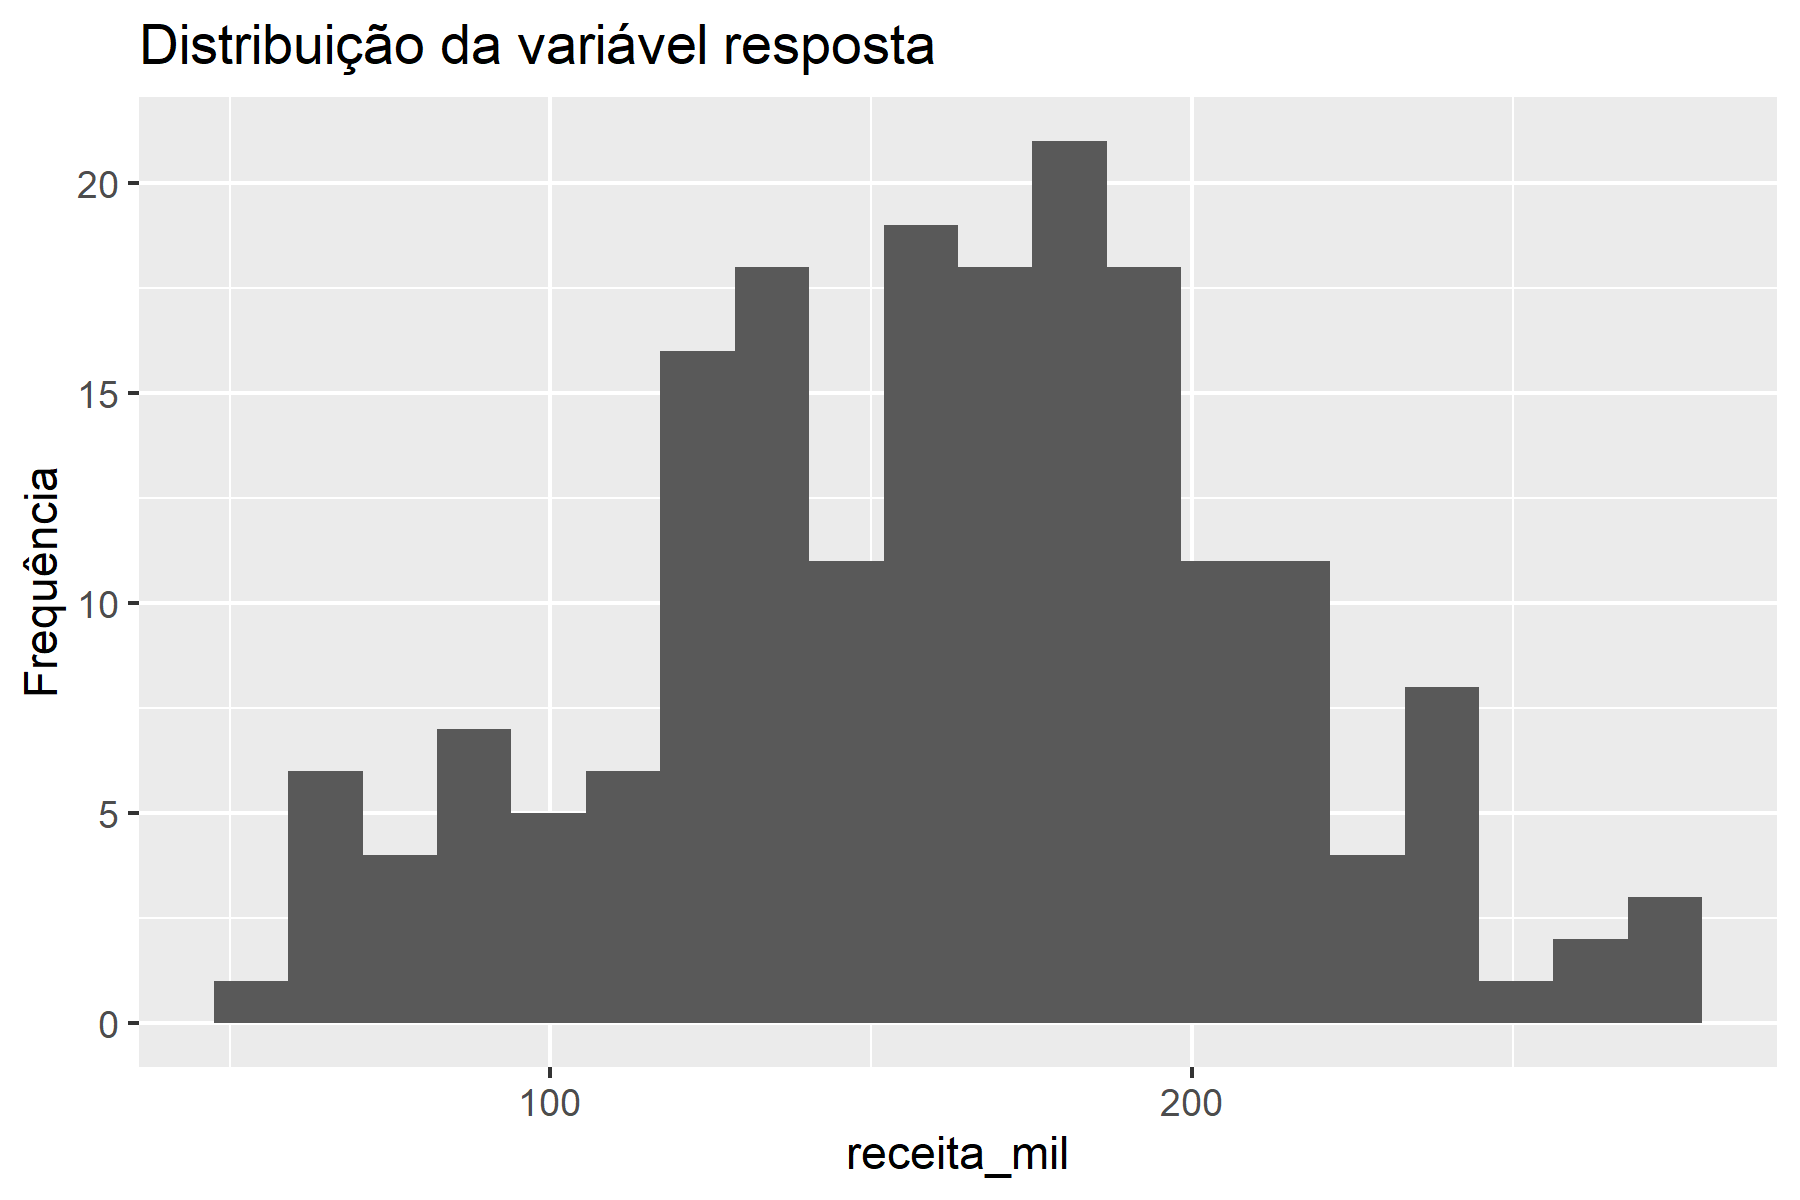
\includegraphics[width=0.7\textwidth]{figures/hist_resposta.png}
\caption{Distribuição da variável receita\_mil}
\end{figure}

\subsection{Boxplot da receita por número de promotores}

\begin{figure}[H]
\centering
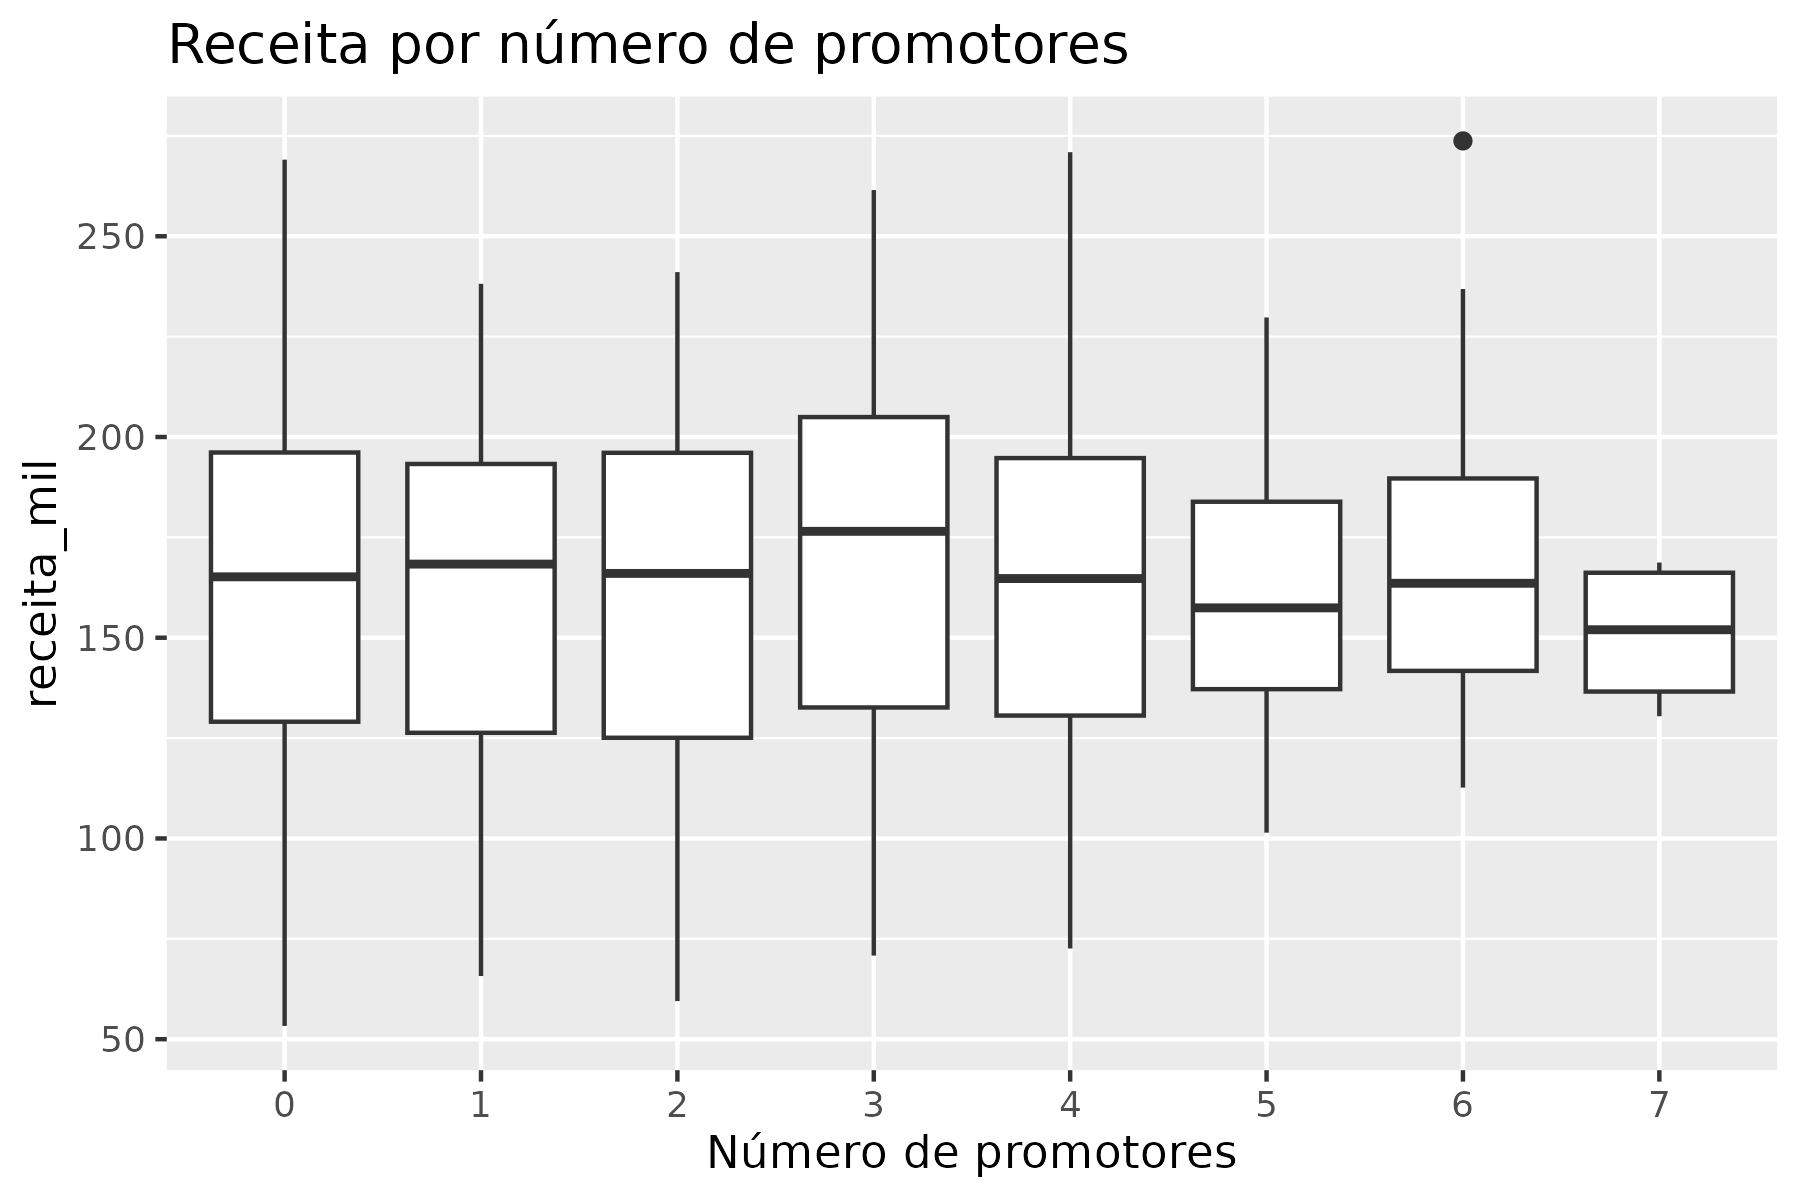
\includegraphics[width=0.7\textwidth]{figures/boxplot_receita_promotores.png}
\caption{Distribuição da receita por número de promotores}
\end{figure}

\subsection{Matriz de correlação}

\begin{figure}[H]
\centering
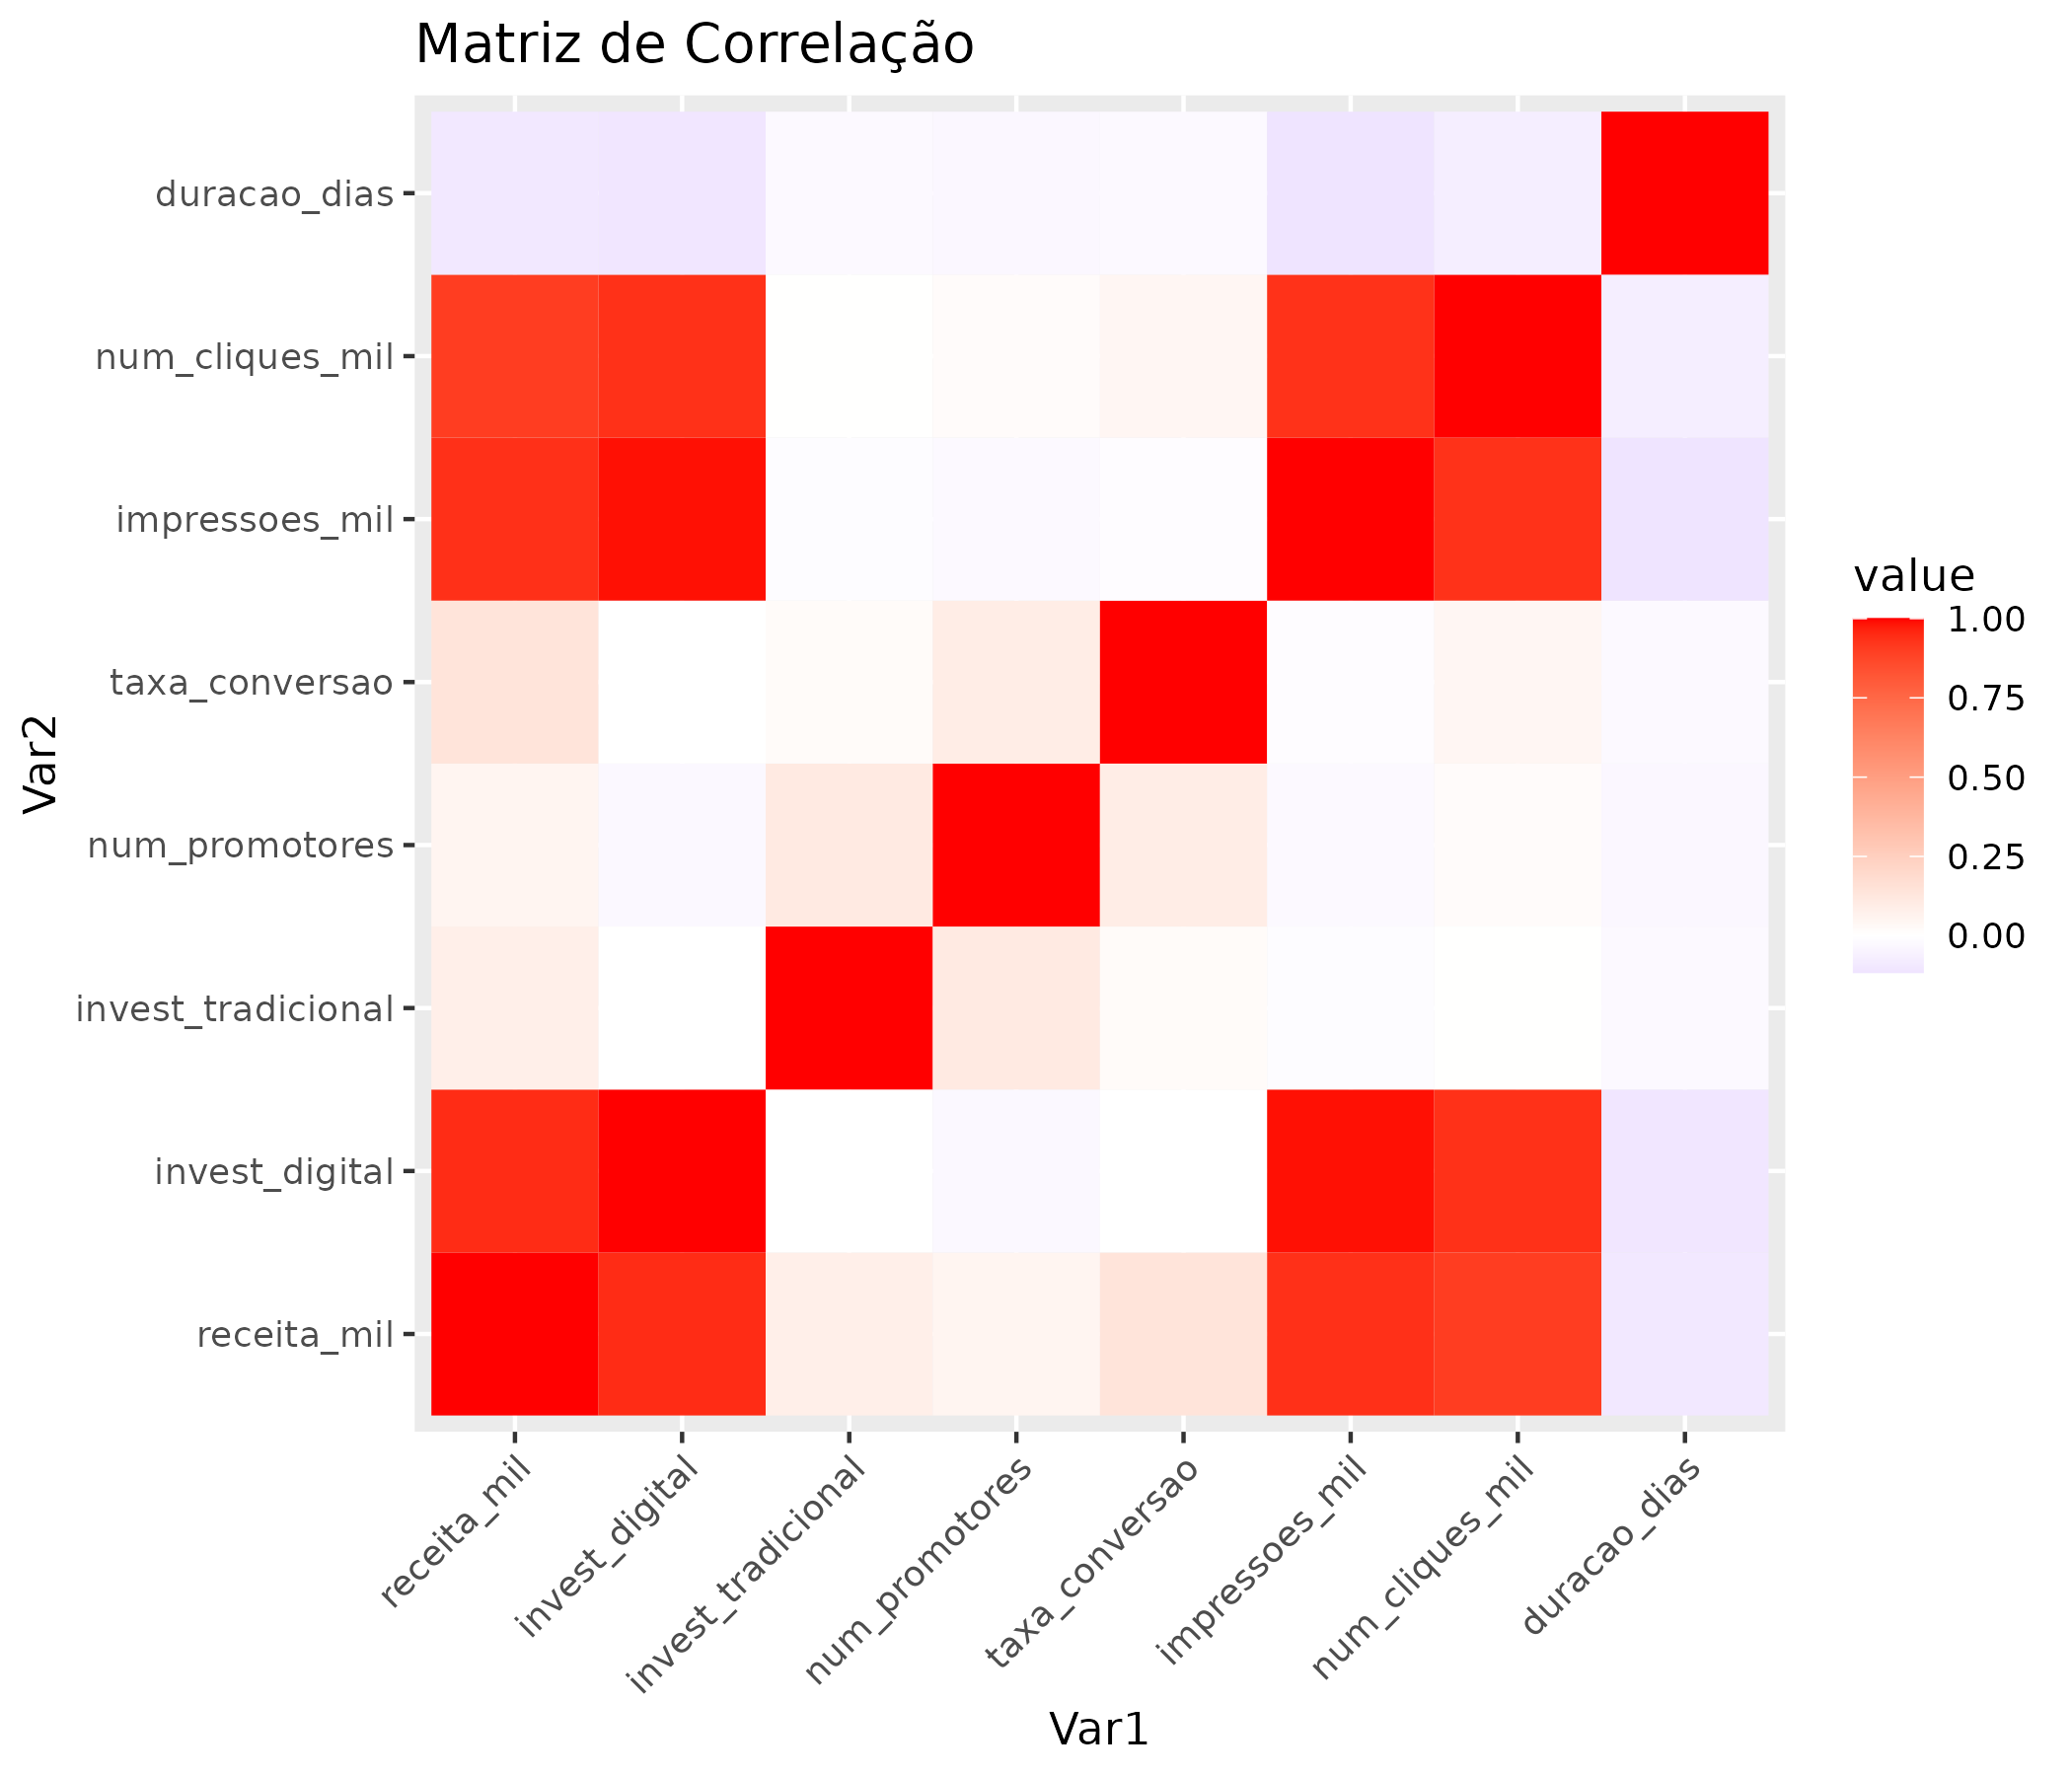
\includegraphics[width=0.7\textwidth]{figures/correlation_heatmap.png}
\caption{Matriz de correlação entre variáveis numéricas}
\end{figure}

A matriz de correlação permite identificar possíveis relações
lineares entre as variáveis explicativas e a variável resposta,
além de indicar possíveis problemas de multicolinearidade.

%%%%%%%%%%%%%%%%%%%%%%%%%%%%%%%%%%%%%%%%%%%%%%%%%%%%
\section{Modelo Inicial de Regressão Linear}

O modelo inicial ajustado foi:

\[
receita\_mil =
\beta_0 +
\beta_1 invest\_digital +
\beta_2 invest\_tradicional +
\beta_3 impressoes\_mil +
\beta_4 num\_cliques\_mil +
\beta_5 taxa\_conversao +
\beta_6 num\_promotores +
\beta_7 duracao\_dias + \varepsilon
\]

\subsection{Coeficientes estimados do modelo final selecionado}

\begin{table}[H]
\centering
\caption{Coeficientes estimados do modelo final selecionado}
% latex table generated in R 4.3.3 by xtable 1.8-4 package
% Sun Mar 15 19:43:47 2026
\begin{table}[ht]
\centering
\begin{tabular}{lrrrr}
  \hline
term & estimate & std.error & statistic & p.value \\ 
  \hline
(Intercept) & 29.88 & 5.48 & 5.45 & 0.00 \\ 
  invest\_digital & 3.18 & 0.57 & 5.56 & 0.00 \\ 
  invest\_tradicional & 0.77 & 0.20 & 3.76 & 0.00 \\ 
  num\_promotores & 1.36 & 0.51 & 2.66 & 0.01 \\ 
  taxa\_conversao & 7.90 & 1.22 & 6.46 & 0.00 \\ 
  impressoes\_mil & 0.03 & 0.03 & 0.82 & 0.41 \\ 
  num\_cliques\_mil & 0.26 & 0.21 & 1.27 & 0.20 \\ 
  duracao\_dias & 0.03 & 0.06 & 0.53 & 0.60 \\ 
   \hline
\end{tabular}
\end{table}

\end{table}

A Tabela apresenta os coeficientes do \textbf{modelo final selecionado}
na etapa de seleção de variáveis (não do modelo inicial completo).

Os coeficientes estimados indicam a variação esperada
na variável resposta para uma unidade adicional de cada
variável explicativa, mantendo as demais constantes.

%%%%%%%%%%%%%%%%%%%%%%%%%%%%%%%%%%%%%%%%%%%%%%%%%%%%
\section{Diagnóstico do Modelo}

Após o ajuste do modelo, foram realizadas análises
de diagnóstico para verificar se os pressupostos
da regressão linear múltipla são atendidos.

\subsection{Resíduos versus valores ajustados}

\begin{figure}[H]
\centering
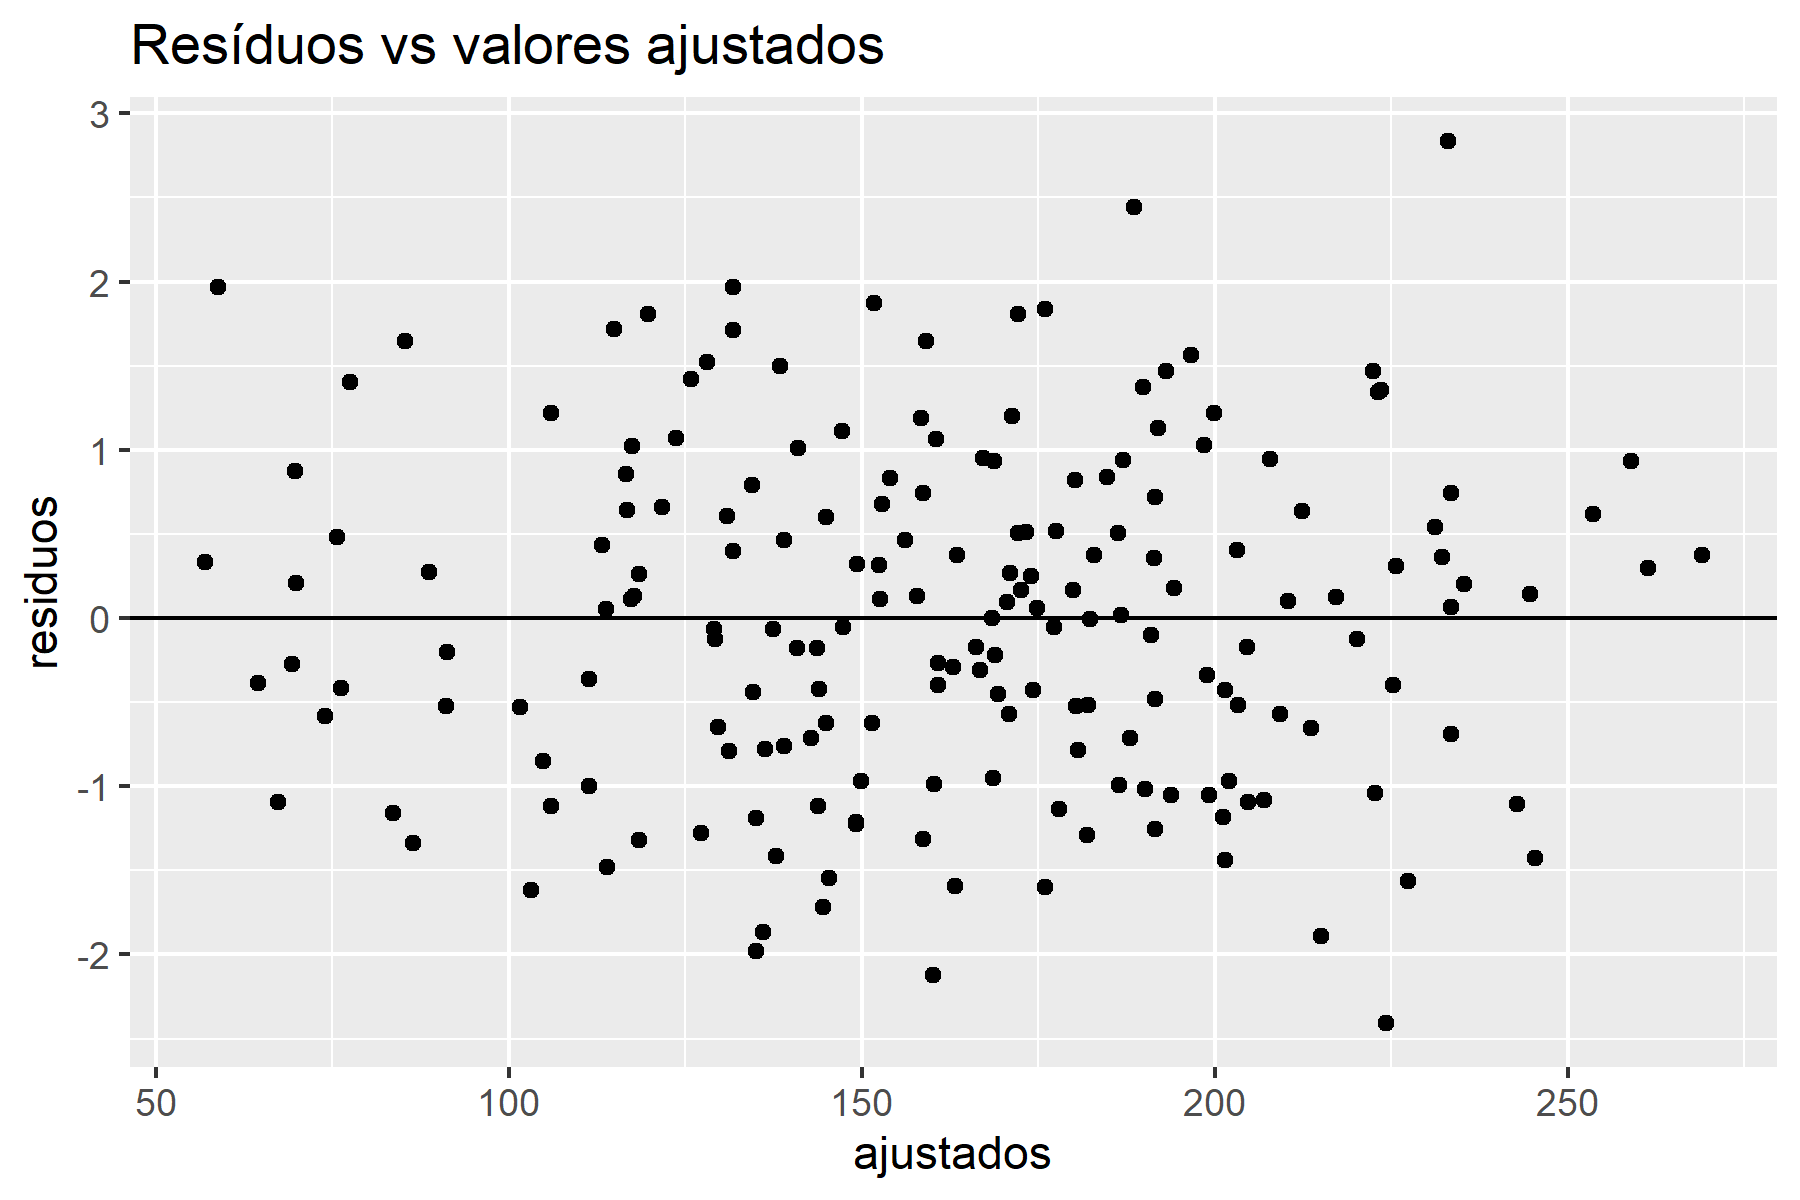
\includegraphics[width=0.7\textwidth]{figures/residuos_vs_ajustados.png}
\caption{Resíduos versus valores ajustados}
\end{figure}

Esse gráfico permite avaliar a presença de padrões
que possam indicar problemas de especificação do modelo.

\subsection{Normalidade dos resíduos}

\begin{figure}[H]
\centering
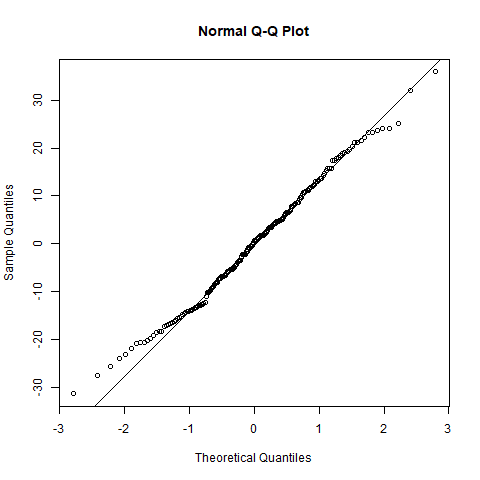
\includegraphics[width=0.7\textwidth]{figures/qqplot_residuos.png}
\caption{Gráfico Q-Q dos resíduos}
\end{figure}

A proximidade dos pontos à linha de referência sugere
que a hipótese de normalidade dos resíduos é razoável.

\subsection{Testes formais de pressupostos}

\begin{table}[H]
\centering
\caption{Resultados dos testes de pressupostos}
% latex table generated in R 4.3.3 by xtable 1.8-4 package
% Sun Mar 15 19:43:47 2026
\begin{table}[ht]
\centering
\begin{tabular}{lr}
  \hline
metrica & valor \\ 
  \hline
Breusch-Pagan p-valor & 0.94 \\ 
  Durbin-Watson p-valor & 0.84 \\ 
  Shapiro-Wilk p-valor & 0.46 \\ 
   \hline
\end{tabular}
\end{table}

\end{table}

Além dos testes de heterocedasticidade e independência,
foi incluído o teste de Shapiro-Wilk para avaliação formal
da normalidade dos resíduos.

\subsection{Diagnóstico de multicolinearidade}

\begin{table}[H]
\centering
\caption{Valores do fator de inflação da variância (VIF)}
% latex table generated in R 4.3.3 by xtable 1.8-4 package
% Sun Mar 15 19:43:47 2026
\begin{table}[ht]
\centering
\begin{tabular}{lr}
  \hline
variavel & vif \\ 
  \hline
invest\_digital & 46.39 \\ 
  invest\_tradicional & 1.02 \\ 
  num\_promotores & 1.04 \\ 
  taxa\_conversao & 1.03 \\ 
  impressoes\_mil & 45.03 \\ 
  num\_cliques\_mil & 8.38 \\ 
  duracao\_dias & 1.03 \\ 
   \hline
\end{tabular}
\end{table}

\end{table}

Valores elevados de VIF podem indicar problemas
de multicolinearidade entre as variáveis explicativas.

%%%%%%%%%%%%%%%%%%%%%%%%%%%%%%%%%%%%%%%%%%%%%%%%%%%%
\section{Observações Influentes}

\begin{figure}[H]
\centering
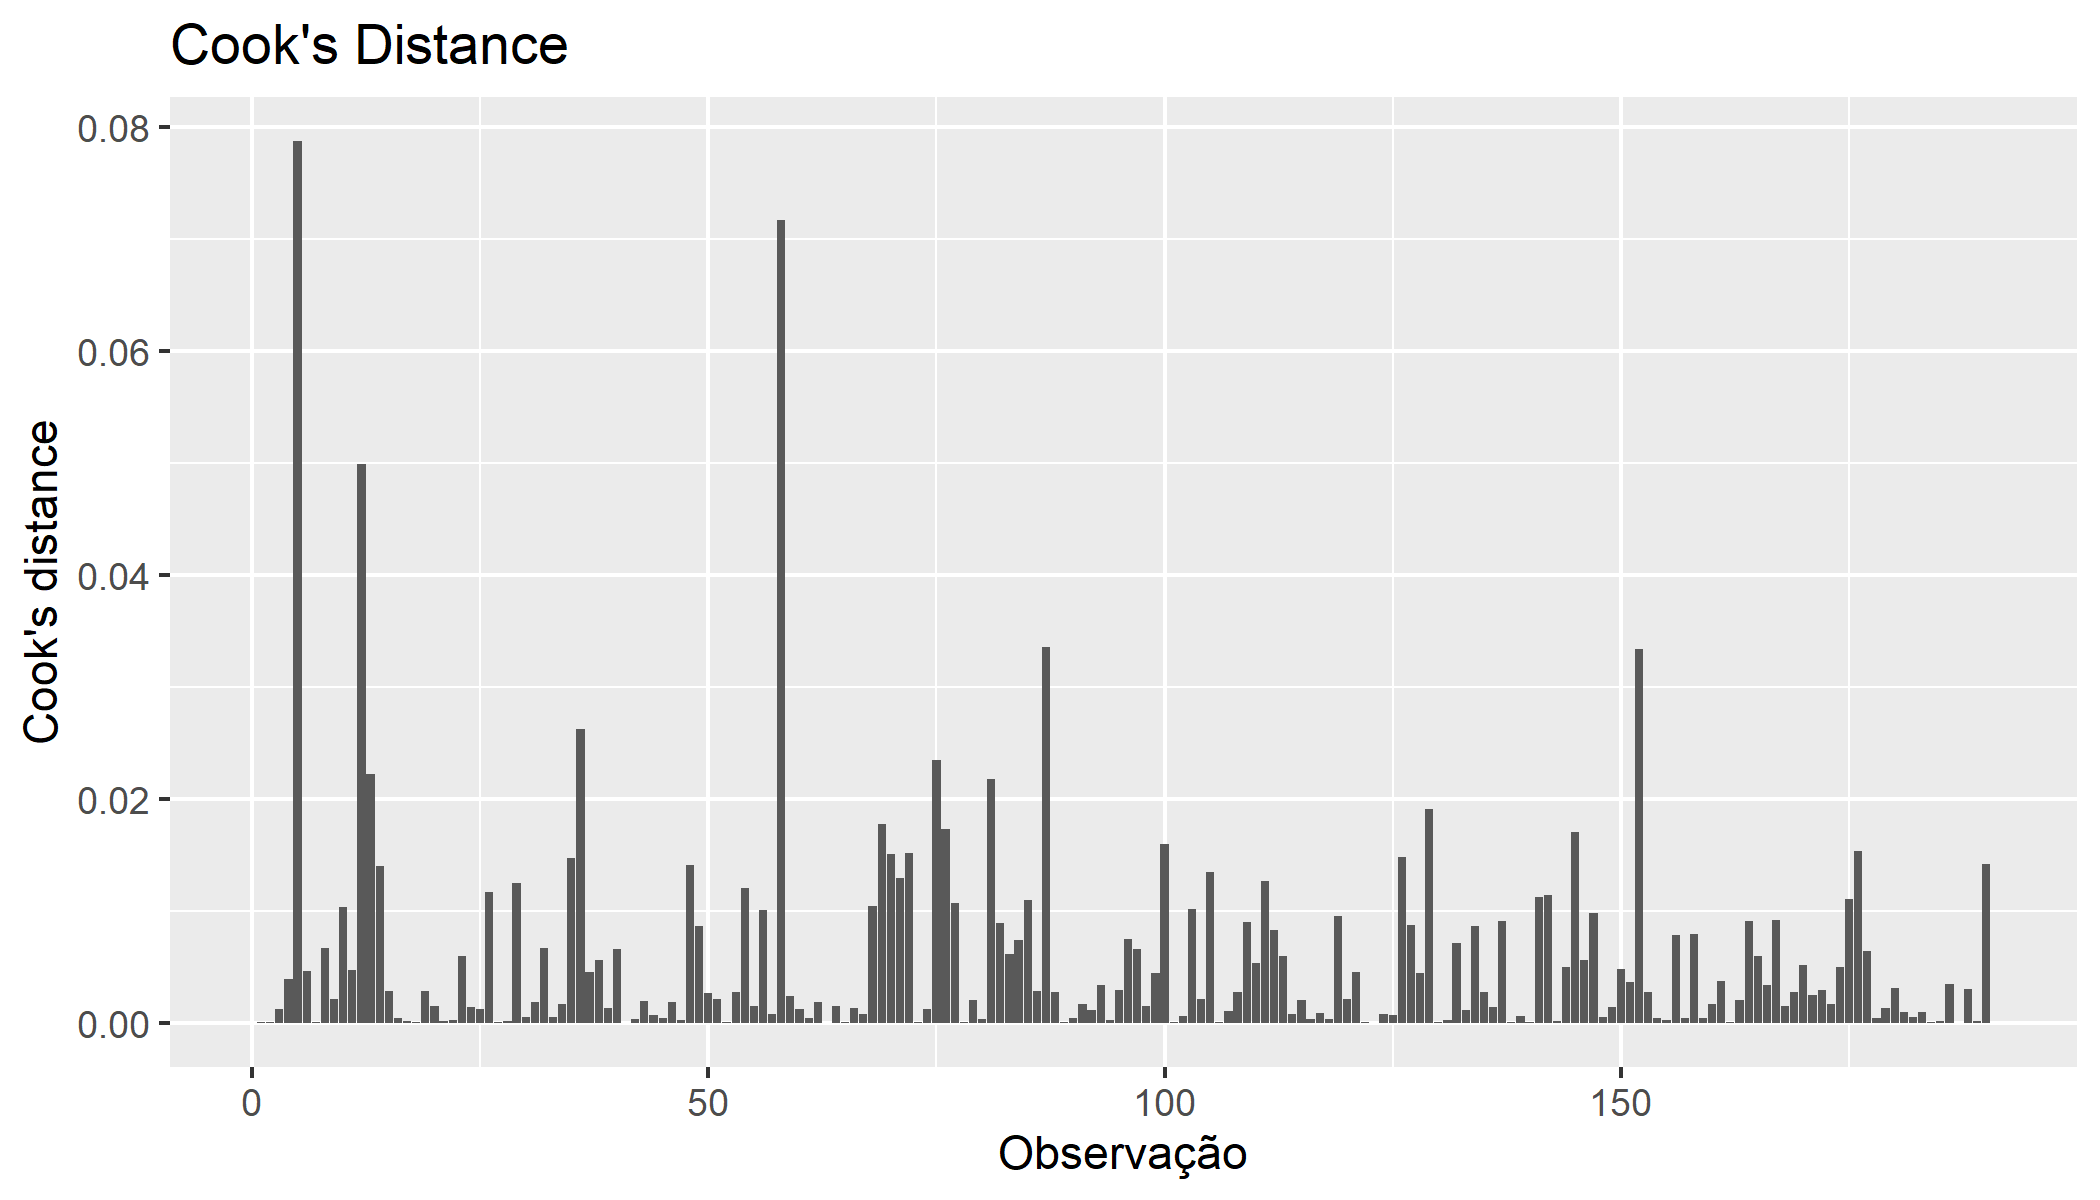
\includegraphics[width=0.7\textwidth]{figures/cooks_distance.png}
\caption{Cook's Distance}
\end{figure}

A análise da distância de Cook permite identificar
observações potencialmente influentes no ajuste do modelo.

%%%%%%%%%%%%%%%%%%%%%%%%%%%%%%%%%%%%%%%%%%%%%%%%%%%%
\section{Previsões e Intervalos}

Foram considerados dois cenários de valores para as
variáveis explicativas com o objetivo de ilustrar
a capacidade de previsão do modelo ajustado.

\begin{table}[H]
\centering
\caption{Tabela 6 -- Cenários de previsão com valores de entrada de $x_1$ e $x_2$}
% latex table generated in R 4.3.3 by xtable 1.8-4 package
% Sun Mar 15 19:43:47 2026
\begin{table}[ht]
\centering
\begin{tabular}{lrrll}
  \hline
cenario & x\_1 & x\_2 & variavel\_x\_1 & variavel\_x\_2 \\ 
  \hline
cenario\_1 & 30.50 & 12.50 & invest\_digital & invest\_tradicional \\ 
  cenario\_2 & 22.25 & 14.65 & invest\_digital & invest\_tradicional \\ 
   \hline
\end{tabular}
\end{table}

\end{table}

Na tabela, $x_1$ e $x_2$ representam, respectivamente,
as duas primeiras variáveis explicativas do modelo final selecionado.

\begin{table}[H]
\centering
\caption{Previsões pontuais e intervalos para os cenários considerados}
% latex table generated in R 4.5.3 by xtable 1.8-8 package
% Sun Mar 15 18:53:19 2026
\begin{table}[ht]
\centering
\begin{tabular}{lrrrrr}
  \hline
cenario & fit & lwr & upr & pred\_lwr & pred\_upr \\ 
  \hline
cenario\_1 & 174.82 & 169.85 & 179.80 & 148.35 & 201.30 \\ 
  cenario\_2 & 147.30 & 142.05 & 152.56 & 120.77 & 173.84 \\ 
   \hline
\end{tabular}
\end{table}

\end{table}

São apresentados intervalos de confiança para a média
esperada da variável resposta e intervalos de predição
para novas observações.

%%%%%%%%%%%%%%%%%%%%%%%%%%%%%%%%%%%%%%%%%%%%%%%%%%%%
\section{Conclusão}

A análise realizada permitiu identificar fatores associados
ao desempenho financeiro das campanhas de marketing.

Os resultados indicam que variáveis relacionadas ao
investimento e ao engajamento digital apresentam maior
associação com a receita obtida pelas campanhas.

Os diagnósticos sugerem que os pressupostos do modelo
de regressão linear múltipla são razoavelmente atendidos,
o que permite utilizar o modelo tanto para interpretação
quanto para previsão.

\end{document}